% Options for packages loaded elsewhere
\PassOptionsToPackage{unicode}{hyperref}
\PassOptionsToPackage{hyphens}{url}
%
\documentclass[
]{article}
\usepackage{amsmath,amssymb}
\usepackage{iftex}
\ifPDFTeX
  \usepackage[T1]{fontenc}
  \usepackage[utf8]{inputenc}
  \usepackage{textcomp} % provide euro and other symbols
\else % if luatex or xetex
  \usepackage{unicode-math} % this also loads fontspec
  \defaultfontfeatures{Scale=MatchLowercase}
  \defaultfontfeatures[\rmfamily]{Ligatures=TeX,Scale=1}
\fi
\usepackage{lmodern}
\ifPDFTeX\else
  % xetex/luatex font selection
\fi
% Use upquote if available, for straight quotes in verbatim environments
\IfFileExists{upquote.sty}{\usepackage{upquote}}{}
\IfFileExists{microtype.sty}{% use microtype if available
  \usepackage[]{microtype}
  \UseMicrotypeSet[protrusion]{basicmath} % disable protrusion for tt fonts
}{}
\makeatletter
\@ifundefined{KOMAClassName}{% if non-KOMA class
  \IfFileExists{parskip.sty}{%
    \usepackage{parskip}
  }{% else
    \setlength{\parindent}{0pt}
    \setlength{\parskip}{6pt plus 2pt minus 1pt}}
}{% if KOMA class
  \KOMAoptions{parskip=half}}
\makeatother
\usepackage{xcolor}
\usepackage[margin=1in]{geometry}
\usepackage{color}
\usepackage{fancyvrb}
\newcommand{\VerbBar}{|}
\newcommand{\VERB}{\Verb[commandchars=\\\{\}]}
\DefineVerbatimEnvironment{Highlighting}{Verbatim}{commandchars=\\\{\}}
% Add ',fontsize=\small' for more characters per line
\usepackage{framed}
\definecolor{shadecolor}{RGB}{248,248,248}
\newenvironment{Shaded}{\begin{snugshade}}{\end{snugshade}}
\newcommand{\AlertTok}[1]{\textcolor[rgb]{0.94,0.16,0.16}{#1}}
\newcommand{\AnnotationTok}[1]{\textcolor[rgb]{0.56,0.35,0.01}{\textbf{\textit{#1}}}}
\newcommand{\AttributeTok}[1]{\textcolor[rgb]{0.13,0.29,0.53}{#1}}
\newcommand{\BaseNTok}[1]{\textcolor[rgb]{0.00,0.00,0.81}{#1}}
\newcommand{\BuiltInTok}[1]{#1}
\newcommand{\CharTok}[1]{\textcolor[rgb]{0.31,0.60,0.02}{#1}}
\newcommand{\CommentTok}[1]{\textcolor[rgb]{0.56,0.35,0.01}{\textit{#1}}}
\newcommand{\CommentVarTok}[1]{\textcolor[rgb]{0.56,0.35,0.01}{\textbf{\textit{#1}}}}
\newcommand{\ConstantTok}[1]{\textcolor[rgb]{0.56,0.35,0.01}{#1}}
\newcommand{\ControlFlowTok}[1]{\textcolor[rgb]{0.13,0.29,0.53}{\textbf{#1}}}
\newcommand{\DataTypeTok}[1]{\textcolor[rgb]{0.13,0.29,0.53}{#1}}
\newcommand{\DecValTok}[1]{\textcolor[rgb]{0.00,0.00,0.81}{#1}}
\newcommand{\DocumentationTok}[1]{\textcolor[rgb]{0.56,0.35,0.01}{\textbf{\textit{#1}}}}
\newcommand{\ErrorTok}[1]{\textcolor[rgb]{0.64,0.00,0.00}{\textbf{#1}}}
\newcommand{\ExtensionTok}[1]{#1}
\newcommand{\FloatTok}[1]{\textcolor[rgb]{0.00,0.00,0.81}{#1}}
\newcommand{\FunctionTok}[1]{\textcolor[rgb]{0.13,0.29,0.53}{\textbf{#1}}}
\newcommand{\ImportTok}[1]{#1}
\newcommand{\InformationTok}[1]{\textcolor[rgb]{0.56,0.35,0.01}{\textbf{\textit{#1}}}}
\newcommand{\KeywordTok}[1]{\textcolor[rgb]{0.13,0.29,0.53}{\textbf{#1}}}
\newcommand{\NormalTok}[1]{#1}
\newcommand{\OperatorTok}[1]{\textcolor[rgb]{0.81,0.36,0.00}{\textbf{#1}}}
\newcommand{\OtherTok}[1]{\textcolor[rgb]{0.56,0.35,0.01}{#1}}
\newcommand{\PreprocessorTok}[1]{\textcolor[rgb]{0.56,0.35,0.01}{\textit{#1}}}
\newcommand{\RegionMarkerTok}[1]{#1}
\newcommand{\SpecialCharTok}[1]{\textcolor[rgb]{0.81,0.36,0.00}{\textbf{#1}}}
\newcommand{\SpecialStringTok}[1]{\textcolor[rgb]{0.31,0.60,0.02}{#1}}
\newcommand{\StringTok}[1]{\textcolor[rgb]{0.31,0.60,0.02}{#1}}
\newcommand{\VariableTok}[1]{\textcolor[rgb]{0.00,0.00,0.00}{#1}}
\newcommand{\VerbatimStringTok}[1]{\textcolor[rgb]{0.31,0.60,0.02}{#1}}
\newcommand{\WarningTok}[1]{\textcolor[rgb]{0.56,0.35,0.01}{\textbf{\textit{#1}}}}
\usepackage{graphicx}
\makeatletter
\def\maxwidth{\ifdim\Gin@nat@width>\linewidth\linewidth\else\Gin@nat@width\fi}
\def\maxheight{\ifdim\Gin@nat@height>\textheight\textheight\else\Gin@nat@height\fi}
\makeatother
% Scale images if necessary, so that they will not overflow the page
% margins by default, and it is still possible to overwrite the defaults
% using explicit options in \includegraphics[width, height, ...]{}
\setkeys{Gin}{width=\maxwidth,height=\maxheight,keepaspectratio}
% Set default figure placement to htbp
\makeatletter
\def\fps@figure{htbp}
\makeatother
\setlength{\emergencystretch}{3em} % prevent overfull lines
\providecommand{\tightlist}{%
  \setlength{\itemsep}{0pt}\setlength{\parskip}{0pt}}
\setcounter{secnumdepth}{-\maxdimen} % remove section numbering
\usepackage{booktabs}
\usepackage{longtable}
\usepackage{array}
\usepackage{multirow}
\usepackage{wrapfig}
\usepackage{float}
\usepackage{colortbl}
\usepackage{pdflscape}
\usepackage{tabu}
\usepackage{threeparttable}
\usepackage{threeparttablex}
\usepackage[normalem]{ulem}
\usepackage{makecell}
\usepackage{xcolor}
\ifLuaTeX
  \usepackage{selnolig}  % disable illegal ligatures
\fi
\usepackage{bookmark}
\IfFileExists{xurl.sty}{\usepackage{xurl}}{} % add URL line breaks if available
\urlstyle{same}
\hypersetup{
  pdftitle={week6HW},
  pdfauthor={Kyle Bosworth},
  hidelinks,
  pdfcreator={LaTeX via pandoc}}

\title{week6HW}
\author{Kyle Bosworth}
\date{2024-10-08}

\begin{document}
\maketitle

{
\setcounter{tocdepth}{2}
\tableofcontents
}
\subsubsection{Load libraries}\label{load-libraries}

\begin{Shaded}
\begin{Highlighting}[]
\FunctionTok{library}\NormalTok{(tidyverse)}
\FunctionTok{library}\NormalTok{(here)}
\FunctionTok{library}\NormalTok{(ggplot2)}
\FunctionTok{library}\NormalTok{(kableExtra)}
\FunctionTok{library}\NormalTok{(prettydoc)}
\end{Highlighting}
\end{Shaded}

\subsubsection{Load and clean up data}\label{load-and-clean-up-data}

\begin{Shaded}
\begin{Highlighting}[]
\NormalTok{maunaluaSGD}\OtherTok{\textless{}{-}}\FunctionTok{read.csv}\NormalTok{(}\FunctionTok{here}\NormalTok{(}\StringTok{"week6"}\NormalTok{,}\StringTok{"data"}\NormalTok{,}\StringTok{"chemicaldata\_maunalua.csv"}\NormalTok{))}
\CommentTok{\#Define the zones in order}
\NormalTok{zone\_order}\OtherTok{\textless{}{-}} \FunctionTok{c}\NormalTok{(}\StringTok{"Near Spring"}\NormalTok{,}\StringTok{"Channel"}\NormalTok{,}\StringTok{"Diffuse"}\NormalTok{,}\StringTok{"Transition"}\NormalTok{,}\StringTok{"Ambient"}\NormalTok{,}\StringTok{"Offshore"}\NormalTok{)}
\CommentTok{\#create as factor}
\NormalTok{maunaluaSGD }\OtherTok{\textless{}{-}}\NormalTok{ maunaluaSGD }\SpecialCharTok{\%\textgreater{}\%}
  \FunctionTok{drop\_na}\NormalTok{(percent\_sgd, Salinity, Zone, Season) }\SpecialCharTok{\%\textgreater{}\%}
  \FunctionTok{mutate}\NormalTok{(}\AttributeTok{Zone =} \FunctionTok{factor}\NormalTok{(Zone, }\AttributeTok{levels =}\NormalTok{ zone\_order))}
\end{Highlighting}
\end{Shaded}

\subsubsection{Inspect the data}\label{inspect-the-data}

\begin{Shaded}
\begin{Highlighting}[]
\FunctionTok{glimpse}\NormalTok{(maunaluaSGD)}
\end{Highlighting}
\end{Shaded}

\begin{verbatim}
## Rows: 340
## Columns: 15
## $ Waypoint    <int> 1, 2, 3, 4, 5, 6, 7, 8, 9, 10, 11, 12, 13, 14, 15, 16, 17,~
## $ Zone        <fct> Transition, Transition, Transition, Transition, Diffuse, D~
## $ Lat         <dbl> 21.27531, 21.27523, 21.27504, 21.27449, 21.27503, 21.27485~
## $ Long        <dbl> -157.7618, -157.7627, -157.7633, -157.7640, -157.7617, -15~
## $ Site        <chr> "W", "W", "W", "W", "W", "W", "W", "W", "W", "W", "W", "W"~
## $ Season      <chr> "SPRING", "SPRING", "SPRING", "SPRING", "SPRING", "SPRING"~
## $ Tide_time   <chr> "Low_Day", "Low_Day", "Low_Day", "Low_Day", "Low_Day", "Lo~
## $ Temp_in     <dbl> 23.75506, 23.53256, 22.63450, 24.01982, 23.26102, 24.00517~
## $ Salinity    <dbl> 27.74029, 30.61192, 28.37008, 32.82124, 29.12293, 34.02018~
## $ Phosphate   <dbl> 0.54, 0.36, 0.50, 0.25, 0.50, 0.13, 0.28, 0.15, 0.23, 0.11~
## $ Silicate    <dbl> 157.93, 92.59, 143.60, 42.32, 126.47, 15.04, 56.31, 23.10,~
## $ NN          <dbl> 7.92, 3.37, 7.29, 0.79, 7.45, 0.46, 1.59, 0.34, 1.91, 0.25~
## $ pH          <dbl> 7.909, 7.965, 8.023, 7.995, 8.005, 8.019, 8.003, 7.978, 7.~
## $ TA          <dbl> 2161.482, 2145.828, 2272.391, 2219.583, 2151.826, 2216.758~
## $ percent_sgd <dbl> 20.4043928, 11.9625323, 18.5529716, 5.4677003, 16.3397933,~
\end{verbatim}

\subsubsection{\texorpdfstring{\emph{What is the relationship between
percent Submarine Groud Water Discharge (SGD) and salinity across
different coastal zones, and how does this relationship vary by
season?}}{What is the relationship between percent Submarine Groud Water Discharge (SGD) and salinity across different coastal zones, and how does this relationship vary by season?}}\label{what-is-the-relationship-between-percent-submarine-groud-water-discharge-sgd-and-salinity-across-different-coastal-zones-and-how-does-this-relationship-vary-by-season}

\subsubsection{Figure 1. Relationship between Percent SGD and Salinity
Across Coastal Zones in Fall and
Spring}\label{figure-1.-relationship-between-percent-sgd-and-salinity-across-coastal-zones-in-fall-and-spring}

\begin{Shaded}
\begin{Highlighting}[]
\FunctionTok{ggplot}\NormalTok{(maunaluaSGD,}
       \FunctionTok{aes}\NormalTok{(}\AttributeTok{x =}\NormalTok{ percent\_sgd,}
           \AttributeTok{y =}\NormalTok{ Salinity,}
           \AttributeTok{color =}\NormalTok{ Zone,}
           \AttributeTok{shape =}\NormalTok{ Season)) }\SpecialCharTok{+} 
  \FunctionTok{geom\_point}\NormalTok{(}\AttributeTok{size =} \DecValTok{3}\NormalTok{, }\AttributeTok{alpha =} \FloatTok{0.7}\NormalTok{) }\SpecialCharTok{+}
  \FunctionTok{geom\_smooth}\NormalTok{(}\AttributeTok{method =} \StringTok{"lm"}\NormalTok{, }\AttributeTok{se =} \ConstantTok{FALSE}\NormalTok{, }
              \FunctionTok{aes}\NormalTok{(}\AttributeTok{group =} \DecValTok{1}\NormalTok{, }
                  \AttributeTok{color =} \StringTok{"black"}\NormalTok{, }
                  \AttributeTok{linetype =} \StringTok{"dashed"}\NormalTok{)) }\SpecialCharTok{+}
  \FunctionTok{scale\_color\_viridis\_d}\NormalTok{() }\SpecialCharTok{+}
    \FunctionTok{facet\_wrap}\NormalTok{(}\SpecialCharTok{\textasciitilde{}}\NormalTok{ Season, }\AttributeTok{scales =} \StringTok{"free"}\NormalTok{) }\SpecialCharTok{+}
    \FunctionTok{labs}\NormalTok{(}\AttributeTok{title =} \StringTok{"Percent SGD and Salinity"}\NormalTok{,}
         \AttributeTok{subtitle =} \StringTok{"[Accross different zones and seasons in Maunalua Bay]"}\NormalTok{,}
         \AttributeTok{x =} \StringTok{"Percent SGD"}\NormalTok{,}
         \AttributeTok{y =} \StringTok{"Salinity (ppt)"}\NormalTok{,}
         \AttributeTok{color =} \StringTok{"Zone"}\NormalTok{,}
         \AttributeTok{Shape =} \StringTok{"Season"}\NormalTok{) }\SpecialCharTok{+}
    \FunctionTok{theme\_minimal}\NormalTok{() }\SpecialCharTok{+}
    \FunctionTok{theme}\NormalTok{(}\AttributeTok{legend.position =} \StringTok{"right"}\NormalTok{,}
          \AttributeTok{plot.title =} \FunctionTok{element\_text}\NormalTok{(}\AttributeTok{hjust =} \FloatTok{0.5}\NormalTok{, }\AttributeTok{face =} \StringTok{"bold"}\NormalTok{),}
          \AttributeTok{plot.subtitle =} \FunctionTok{element\_text}\NormalTok{(}\AttributeTok{hjust =} \FloatTok{0.5}\NormalTok{, }\AttributeTok{face =} \StringTok{"italic"}\NormalTok{))}
\end{Highlighting}
\end{Shaded}

\begin{center}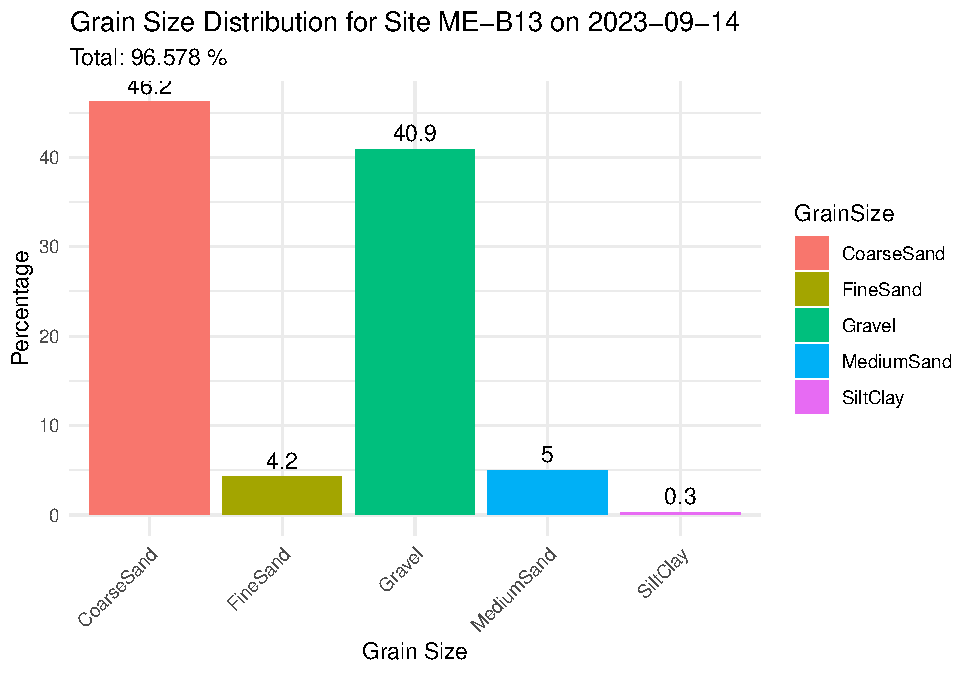
\includegraphics[width=1\linewidth]{week6HW_files/figure-latex/unnamed-chunk-4-1} \end{center}

\subsubsection{Table 1. Mean Salinity and SGD
(Fall)}\label{table-1.-mean-salinity-and-sgd-fall}

\begin{Shaded}
\begin{Highlighting}[]
\NormalTok{fall\_table}\OtherTok{\textless{}{-}}\NormalTok{maunaluaSGD }\SpecialCharTok{\%\textgreater{}\%}
  \FunctionTok{filter}\NormalTok{(Season }\SpecialCharTok{==} \StringTok{"FALL"}\NormalTok{) }\SpecialCharTok{\%\textgreater{}\%}
  \FunctionTok{group\_by}\NormalTok{(Zone) }\SpecialCharTok{\%\textgreater{}\%} 
  \FunctionTok{summarise}\NormalTok{(}
    \AttributeTok{mean\_salinity =} \FunctionTok{mean}\NormalTok{(Salinity),}
    \AttributeTok{mean\_percent\_sgd =} \FunctionTok{mean}\NormalTok{(percent\_sgd)) }\SpecialCharTok{\%\textgreater{}\%}
  \FunctionTok{arrange}\NormalTok{(}\FunctionTok{factor}\NormalTok{(Zone, }\AttributeTok{levels =}\NormalTok{ zone\_order))}

\FunctionTok{kable}\NormalTok{(fall\_table, }\AttributeTok{caption =} \StringTok{"Table 1. Mean Salinity by Zone (Fall)"}\NormalTok{) }\SpecialCharTok{\%\textgreater{}\%}
  \FunctionTok{kable\_styling}\NormalTok{(}\AttributeTok{bootstrap\_options =} \FunctionTok{c}\NormalTok{(}\StringTok{"striped"}\NormalTok{,}
                                      \StringTok{"hover"}\NormalTok{,}
                                      \StringTok{"condensed"}\NormalTok{), }\AttributeTok{full\_width =}\NormalTok{ F)}
\end{Highlighting}
\end{Shaded}

\begin{longtable}[t]{lrr}
\caption{\label{tab:unnamed-chunk-5}Table 1. Mean Salinity by Zone (Fall)}\\
\toprule
Zone & mean\_salinity & mean\_percent\_sgd\\
\midrule
Near Spring & 20.03356 & 48.394028\\
Diffuse & 34.08268 & 1.844870\\
Transition & 33.33047 & 4.058730\\
Ambient & 34.56727 & 0.381286\\
\bottomrule
\end{longtable}

\subsubsection{Table 2. Mean Salinity and SGD
(SPRING)}\label{table-2.-mean-salinity-and-sgd-spring}

\begin{Shaded}
\begin{Highlighting}[]
\NormalTok{spring\_table}\OtherTok{\textless{}{-}}\NormalTok{maunaluaSGD }\SpecialCharTok{\%\textgreater{}\%}
  \FunctionTok{filter}\NormalTok{(Season }\SpecialCharTok{==} \StringTok{"SPRING"}\NormalTok{) }\SpecialCharTok{\%\textgreater{}\%}
  \FunctionTok{group\_by}\NormalTok{(Zone) }\SpecialCharTok{\%\textgreater{}\%}
  \FunctionTok{summarise}\NormalTok{(}
    \AttributeTok{mean\_salinity =} \FunctionTok{mean}\NormalTok{(Salinity),}
    \AttributeTok{mean\_percent\_sgd =} \FunctionTok{mean}\NormalTok{(percent\_sgd)) }\SpecialCharTok{\%\textgreater{}\%}
  \FunctionTok{arrange}\NormalTok{(}\FunctionTok{factor}\NormalTok{(Zone, }\AttributeTok{levels =}\NormalTok{ zone\_order))}

\FunctionTok{kable}\NormalTok{(fall\_table, }\AttributeTok{caption =} \StringTok{"Table 2. Mean Salinity and SGD by Zone (SPRING)"}\NormalTok{) }\SpecialCharTok{\%\textgreater{}\%}
  \FunctionTok{kable\_styling}\NormalTok{(}\AttributeTok{bootstrap\_options =} \FunctionTok{c}\NormalTok{(}\StringTok{"striped"}\NormalTok{, }
                                      \StringTok{"hover"}\NormalTok{, }
                                      \StringTok{"condensed"}\NormalTok{), }\AttributeTok{full\_width =}\NormalTok{ F)}
\end{Highlighting}
\end{Shaded}

\begin{longtable}[t]{lrr}
\caption{\label{tab:unnamed-chunk-6}Table 2. Mean Salinity and SGD by Zone (SPRING)}\\
\toprule
Zone & mean\_salinity & mean\_percent\_sgd\\
\midrule
Near Spring & 20.03356 & 48.394028\\
Diffuse & 34.08268 & 1.844870\\
Transition & 33.33047 & 4.058730\\
Ambient & 34.56727 & 0.381286\\
\bottomrule
\end{longtable}

\end{document}
